\begin{figure}[H]
    \centering
    \definecolor{waterblue}{RGB}{92,185,220}
    \definecolor{pressureblue}{RGB}{30,95,175}
    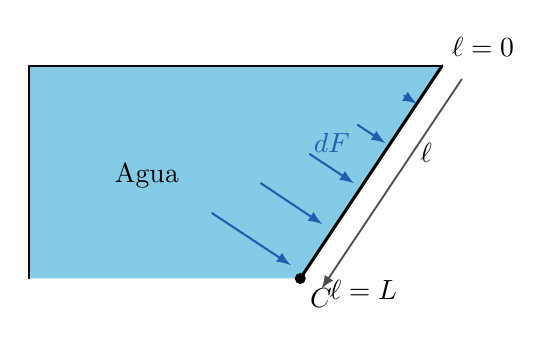
\begin{tikzpicture}[x=1cm,y=1cm,line cap=round,line join=round]
        \coordinate (C) at (4.10,0.35);
        \coordinate (S) at (5.90,3.05);

        % Agua y compuerta
        \fill[waterblue!75] (0.65,0.35) -- (C) -- (S) -- (0.65,3.05) -- cycle;
        \draw[line width=0.7pt] (0.65,0.35) -- (0.65,3.05) -- (S);
        \draw[line width=1.1pt] (C) -- (S);
        \fill (C) circle (0.07);
        \node[below right] at (C) {$C$};
        \node[above right] at (S) {$\ell=0$};
        \node at (2.15,1.65) {Agua};

        % Coordenada a lo largo de la compuerta
        \draw[black!70,-latex,line width=0.65pt]
            (6.15,2.88) -- (4.37,0.22);
        \node[right] at (5.50,1.95) {$\ell$};
        \node[right] at (4.35,0.20) {$\ell=L$};

        % Fuerzas diferenciales: magnitud creciente con la profundidad
        \draw[pressureblue,-latex,line width=0.75pt] (5.42,2.67) -- (5.58,2.57);
        \draw[pressureblue,-latex,line width=0.75pt] (4.83,2.30) -- (5.18,2.07);
        \draw[pressureblue,-latex,line width=0.75pt] (4.22,1.93) -- (4.78,1.56);
        \draw[pressureblue,-latex,line width=0.75pt] (3.60,1.56) -- (4.38,1.04);
        \draw[pressureblue,-latex,line width=0.75pt] (2.98,1.18) -- (3.98,0.52);
        \node[pressureblue,above] at (4.50,1.82) {$dF$};

    \end{tikzpicture}
    \caption{Distribución hidrostática sobre la compuerta, usando $\ell$ desde la superficie libre.}
\end{figure}
